\documentclass{article}
\usepackage[utf8]{inputenc}
\usepackage{listings}
\usepackage{float}
\title{Rakugo Technical Whitepaper}
\author{Rakugo}
\date{July 14 2017}
\setlength{\parskip}{1em}
\usepackage{natbib}
\usepackage{graphicx}
\usepackage{amssymb}
\usepackage{amsmath}
 
\begin{document}

\maketitle

\begin{abstract}
Rakugo revolutionizes online publishing through notarization and monetization on the Ethereum blockchain. When a user publishes content through Rakugo, they are paid royalties for revenue generated by their content and the content is copyrighted through notarization on the Ethereum blockchain. The Rakugo Engine goes further by optimizing royalties through increased user influence and trend creation.

\end{abstract}

\section{Rakugo Platform}
The functionality of the Rakugo platform abstracts crowdsale analytics and interaction with the Ethereum blockchain with an intuitive user interface. Our approach is a web application that combines content management with the functionality of an ethereum wallet. Royalties are generated from published content and distributed to holders of tokens representing online content. Content producers can choose to have funds transferred as USD or as ETH via our royalty distribution model outlined below.


Rakugo creates a digital representation of digital content on the Ethereum blockchain by deploying an ERC20-standard token-creating smart contract with a unique digital fingerprint. Content is notarized by the deployment of the contract and ownership of the content is represented by the ownership of these tokens. The parameters of token creation and ownership structure are supplied by the creator during deployment of the smart contract. Tokens can be traded or held via an ownership model of the creator's choosing. Royalties are generated when content is published through Rakugo and is dispersed based upon the owner's chosen configuration.
The ways in which a creator can issue representations of their content are boundless and Rakugo empowers users to try anything without the burden of writing or deploying code to the Ethereum network. 
Rakugo empowers all creatives with the ability to notarize and monetize their work with the security and accessibility of a distributed ledger that blockchains provide.


\section{Rakugo Assetization}
The crux of Rakugo’s value is our ability to "assetize" or create a digital representation of content on the Ethereum blockchain. These representations are referred to as 'Namespace Tokens', as their publicly accessible name attribute is composed of a logical grouping of unique identifiers.

ERC20-standard 'Namespace Tokens' are created via smart contract, each with an identifying payload that notarizes the content and its creator. Figure 1 schema describes information that will be available after decompression of a token’s digital fingerprint attribute

This JSON object corresponding to the schema above is compressed and added as a public attribute of the token creation contract as the pseudo-solidity code below

\begin{minipage}{\linewidth}
\begin{lstlisting}[language=java]

contract MyToken {

    string public name;
    bytes public digitalFingerprint;

    function MyToken(...) {
        name = "wyatt_meldman-floch.rakugo_whitepaper";
        digitalFingerprint = /compressed json bytes/;
        
    ...
    
    }
}
\end{lstlisting}
\end{minipage}

\section{ERC223 Compatibility}
We are monitoring the ERC223 token standard proposal\footnote{https://github.com/ethereum/EIPs/issues/223} and are factoring future compatibility of into the design of our Namespace tokens.

\section{Rakugo Royalty Distribution}

The Namespace Tokens described above are the tool used to redeem royalties from the Rakugo platform. Royalties (at the owner's choice) can be disbursed to token holders via a smart contract where the token(s) is used to attribute the correct allocation of royalties to its holder. This decentralized approach allows users to freely manage their assets without relying on the Rakugo platform if they so choose. Users also have the ability to automate the royalties distribution through our the Rakugo platform.

This model provides a safer approach to royalty distribution than similar Dapps that rely on a third-party API (such as a block explorer for finding wallet addresses of token holders). Distribution occurs via a handshake where a token(s) is sent to a smart contract and royalties along with the token(s) is sent back to the token holder. Thus if this wallet address is not hosted through our platform we can verify ownership and safely disburse royalties to the rightful owner.

\begin{figure}[H]
\centering
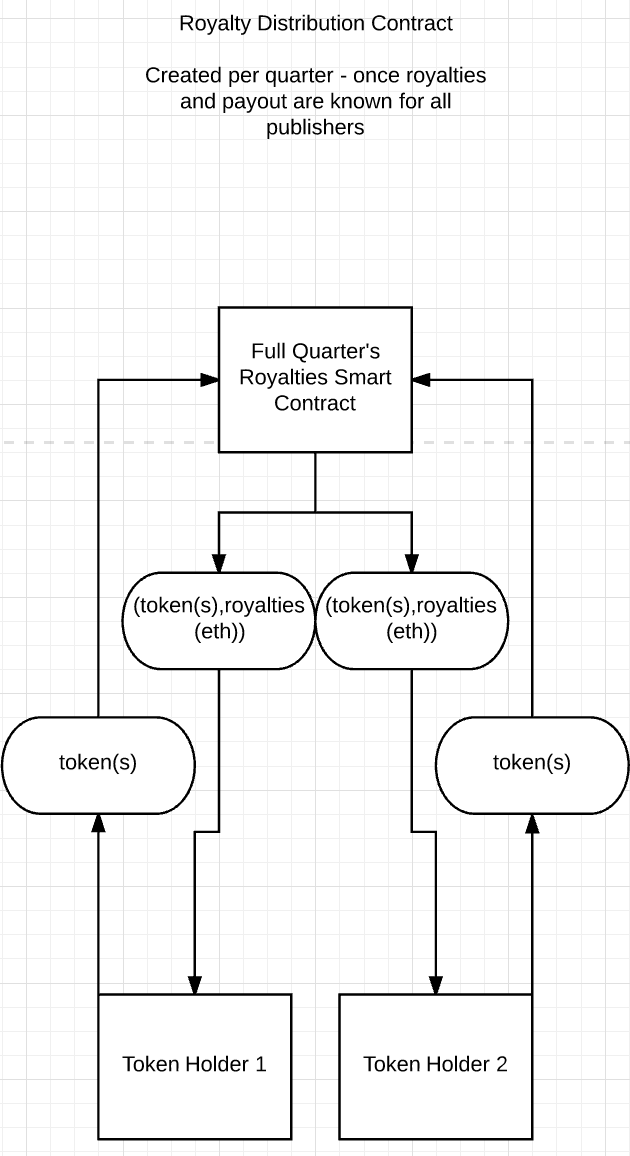
\includegraphics[scale=0.65]{royalty_distro.png}
\caption{Royalty Distribution Architecture}
\end{figure}

\section{Smart Publishing}
As the Rakugo platform grows, we are presented with a unique opportunity to optimize overall royalty generation by leveraging our scale. Below details our approach to scaling the Rakugo Platform and optimizing royalty generation with real-time machine learning.

Rakugo employs a "Smart Publishing" approach to royalty optimization which prioritizes relevance to trending topics on top search engines. Tailoring content to match trending topics increases search engine exposure, royalty generation and overall influence of the content producer. Content is matched to currently trending topics via a proprietary topic modeling algorithm and a suggestions that increase relevance to these topics are provided to the producer. Beyond that, Rakugo seizes opportunities to drive emerging trends, increasing the overall influence and value of the Rakugo platform. 

Trends are identifiable across streams of data using a cross dependence temporal topic model (CDTTM)\footnote{Wang, X., Zhai, C., Hu, X., Sproat, R.: Mining correlated bursty topic patterns from coordinated text streams. In: Proceedings of the 13th ACM International Conference on Knowledge Discovery in Data Mining, pp. 784–793 (2007)}. A cross dependence temporal topic model identifies dependent and temporal correlation across streams streams of data for building correlated generative processes with mutual reinforcement.\footnote{Blei, D.M., Lafferty, J.D.: Dynamic topic models. In: Proceedings of the 23rd International Conference on Machine Learning, pp. 113–120 (2006)}

Consider topic distributions, \begin{math} \theta_1, \theta_2 \end{math} across streams of major news outlet content and Rakugo user generated contend (UGC) where \begin{math} \phi \end{math} denotes the word distribution of each topic; \begin{math} x \end{math} is a binary variable indicating whether the generation of the current word is influenced by
the previous news or UGC \begin{math} (x = 1) \end{math} if so or \begin{math} (x = 0) \end{math} if not. \begin{math} \alpha \end{math}, \begin{math} \beta \end{math} are the Dirichlet hyper
parameters and \begin{math} \lambda \end{math} is the Bernoulli parameter for sampling \begin{math} x \end{math}, \begin{math} \gamma_d \end{math}, \begin{math} \gamma_p \end{math} are its hyper
parameters.

\begin{figure}[H]
\centering
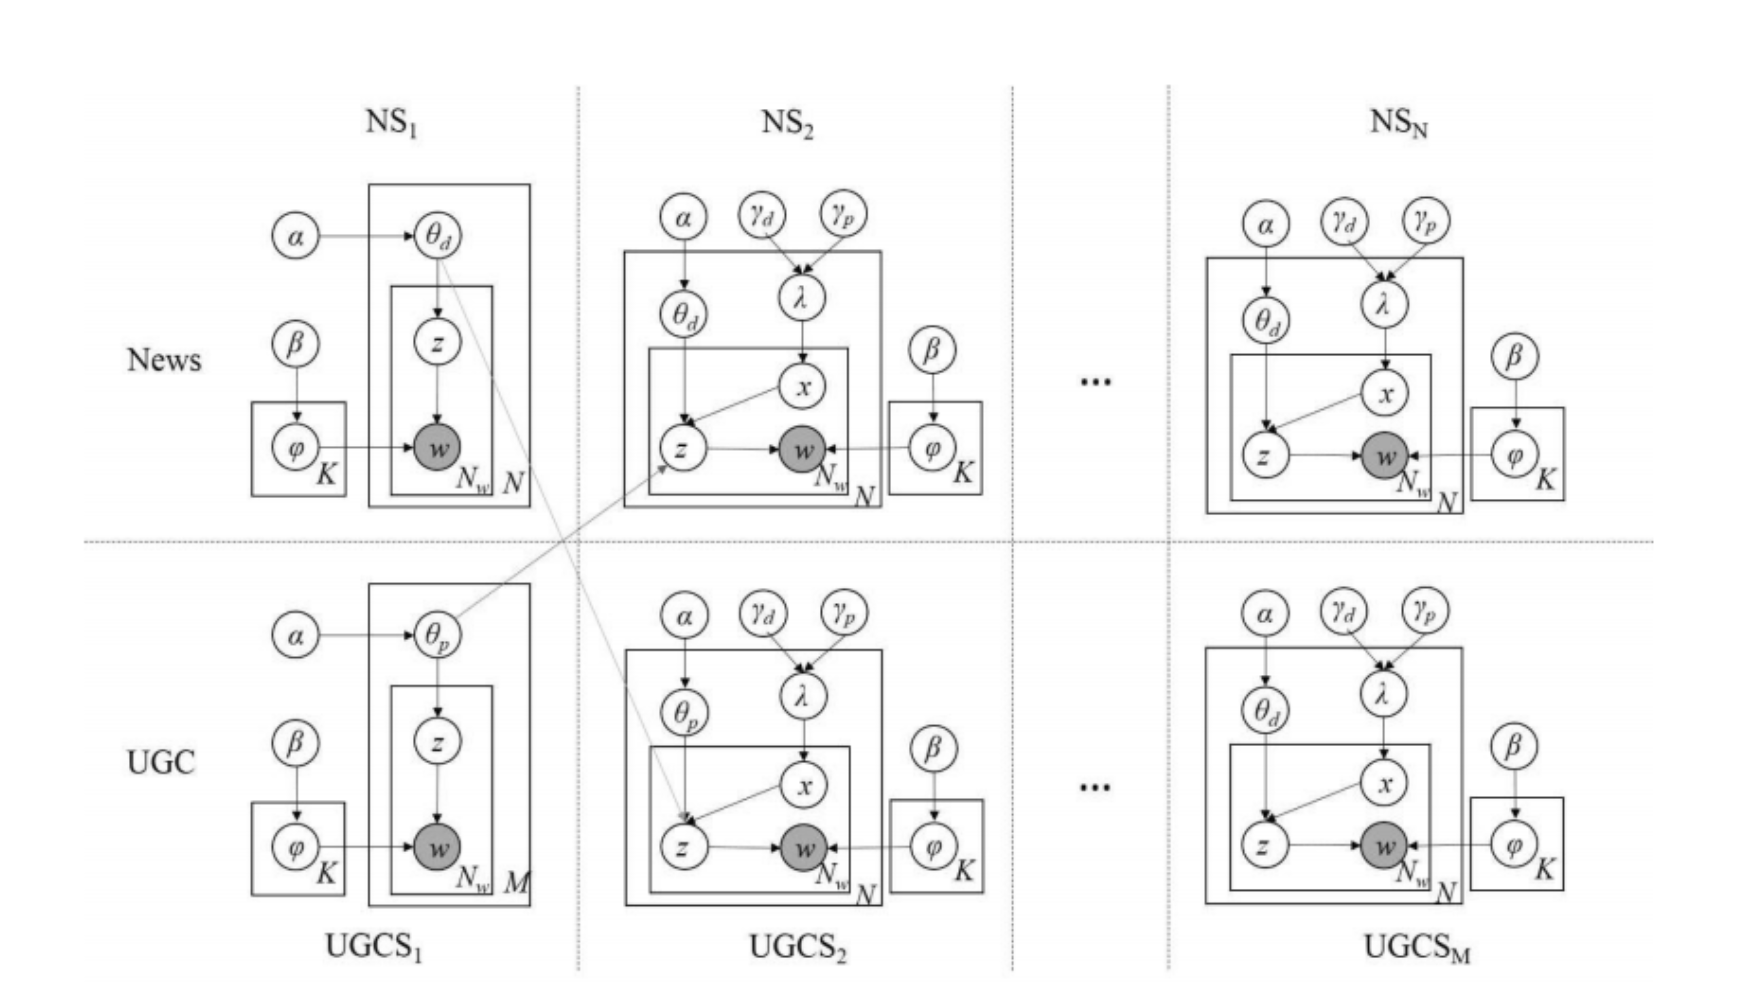
\includegraphics[scale=0.4]{CDTTM.png}
\caption{Cross Dependant Temporal Topic Model\textsuperscript{1}}
\end{figure}

For the generative process, we partition both steams into disjoint substreams with fixed time intervals, e.g. NS = \begin{math} NS_1  \bigcup ... \bigcup NS_n \end{math} where \begin{math} NS_i \end{math} is with time [ti,ti+1), and initialize two standard LDA models in the first substreams \begin{math} NS_1 \end{math} and \begin{math} UGSC_1 \end{math}. As for the subsequent substreams, if there is a previous substream in the other stream (e.g. \begin{math} NSi_1 \end{math} has a previous \begin{math} UGC \end{math} substream \begin{math} UGCS_i \end{math}), a coin x is tossed according to \begin{math} p(x|d) \sim (\gamma_d, \gamma_p \end{math}) to decide whether \begin{math} w_d \end{math} inherits from the previous substream, otherwise (namely when there is no previous substream in the other stream) a standard LDA model can be employed for word sampling. The diagram in Figure 2 graphically describes this algorithm. Further descriptions of similar CDTTM implementations can be found in (Wang, X. et al). 

A CDTTM allows us to quantify topical influence across streams using a common metric in information theory known as Kullback-Leibler(KL) divergence.\footnote{Hou, L., Li, J., Li, X.L., Su, Y.: Measuring the influence from user-generated content to news via cross-dependence topic modeling. International Conference on Database Systems for Advanced Applications, 125-141} If topics $z_{1}$ and $z_{2}$ associated with two distributions \begin{math} \psi_1 \end{math} and \begin{math} \psi_2 \end{math}, influence \begin{math} \zeta_{(z_{1} \rightarrow z_{2}} \end{math} from $z_{1}$ to $z_{2}$ can be defined as the added information content in $z_{1}$ compared to $z_{2}$.

\begin{equation*}
\zeta_{(z_{1} \rightarrow z_{2}} = KL(z_{1} | z_{2}) = \sum^{\nu}_{i=1} \psi_{2i} \times \log \frac{\psi_{2i}}{\psi_{1i}} 
\end{equation*}

Rakugo increases individual influence in two ways: by tailoring individual content to trending topics via a proprietary topic-document similarity score and by optimizing Topic Progressiveness, a metric denoting the possibility of user content triggering trends in major news channels, between the stream of all Rakugo articles with respect to top content sources. For each topic $z_{p}$ in the Rakugo content stream with a corresponding linked topic $L(z_{p})$ in a major content stream, the cross-entropy values are computed to find the minimum \begin{math} z^{min}_{d} \end{math}, and then the Topic Progressiveness is defined as:

\begin{equation*}
Prog(z_{p}) = T(\operatornamewithlimits{argmin}\limits_{z_{d\in L(z_{p})}} H(z_{p}, z_{d})) - T(z_{p})
\end{equation*}

where \begin{math} H(z_{p},z_{d}) \end{math} is the cross-entropy of \begin{math} z_{p} \end{math} to its linked topic \begin{math} z_{d} \end{math} and T denotes the timestamp of the input topic.\textsuperscript{3} Optimization of Topic Progressiveness increases influence of the individual user and the total influence of all Rakugo generated content.

\section{Rakugo Smart Publishing Engine}
The Rakugo Smart Publishing Engine recommends edits to content based upon trending topics identified in real-time. Using the methods described above, our engine performs real-time topic modeling between Rakugo and competing content streams. From the user's perspective we offer on demand edit suggestions to align sentiment to trending topics. A topic similarity score is generated by our matching algorithm between content and trending topics, suggestions to increase topic relevance are then provided to the user. From a macro perspective, our engine provides suggestions to all Rakugo users when the potential to influence the emergence of a trending topic presents itself. Using historical data and currently trending topics identified by our CDTTM platform, edit suggestions are provided in the same manner as our topic relevance score and users are rewarded for their contribution to resultant trends identified by the CDTTM platform after the trend creation campaign.

\begin{figure}[H]
\centering
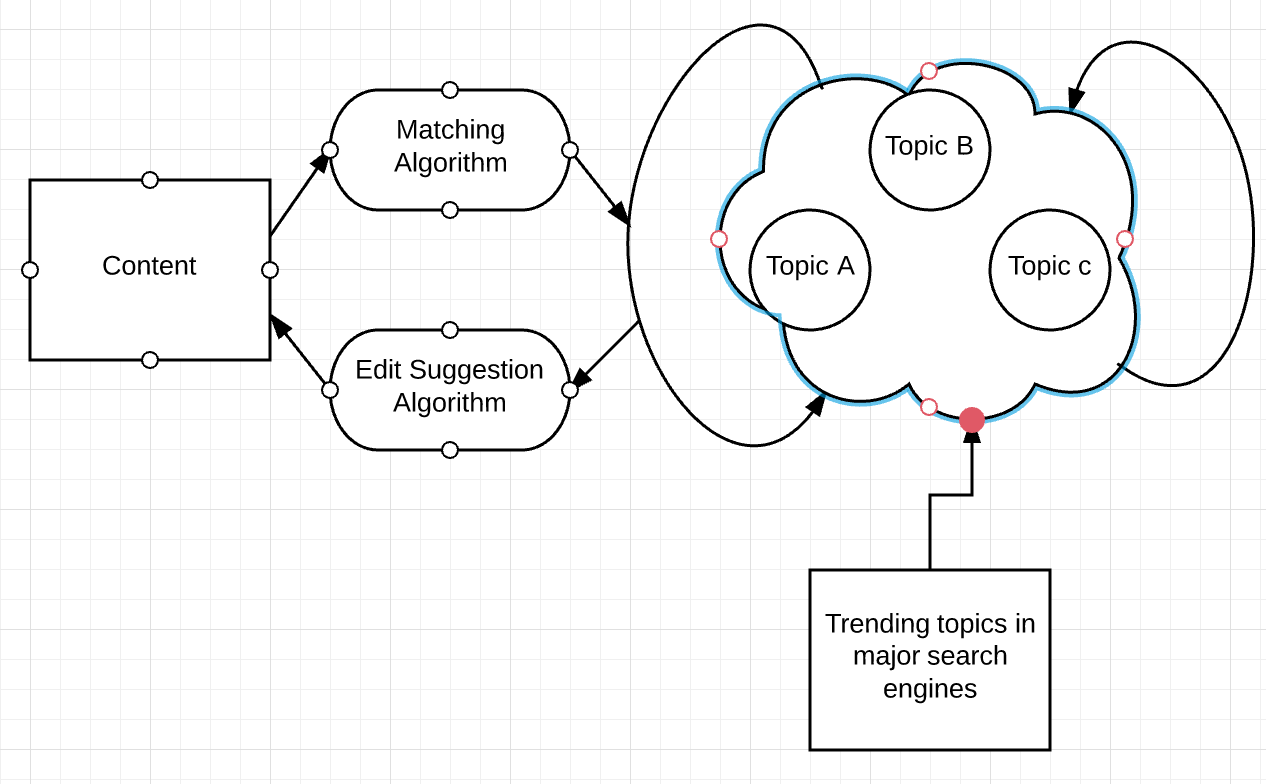
\includegraphics[scale=0.60]{smart_publishing_engine.png}
\caption{Content Editing Architecture}
\end{figure}

\section{Conclusion}
The Rakugo Platform combined with our smart publishing engine provides a next generation approach to content management and publishing. Unlike other applications like Medium, Buzzfeed or Steemit content creators own the rights to their content through copyright and get paid their fair royalties as actual money. Rakugo goes beyond that by optimizing royalty generation, influence and the ability to monetize or share value as the user chooses. These details will be abstracted by an intuitive user interface but will also be accessible to power users via public a API.

\newpage

\renewcommand{\lstlistingname}{Appendix}
\begin{lstlisting}[caption={Digital Fingerprint},captionpos=b, language=java,numbers=none]

{
    "$schema": "digital_fingerprint",
    "definitions": {},
    "id": "https://rakugo.co/whitepaper",
    "properties": {
        "compressedContent": {
            "id": "/properties/compressedContent",
            "items": {
                "id": "/properties/compressedContent/items",
                "type": "integer"
            },
            "type": "array"
        },
        "link": {
            "id": "/properties/link",
            "type": "string"
        },
        "name": {
            "id": "/properties/name",
            "type": "string"
        },
        "publishDate": {
            "id": "/properties/publishDate",
            "type": "string"
        }
    },
    "type": "object"
}

\end{lstlisting}

\bibliographystyle{plain}
\end{document}

